% -----------------------------------------------------------------------------
% Arquivo: ./03-elementos-pos-textuais/apendices.tex
% -----------------------------------------------------------------------------


\begin{apendicesenv}
\partapendices


% -----------------------------------------------------------------------------
% Primeiro apêndice
% -----------------------------------------------------------------------------


\chapter{Nome do apêndice} 			% edite para alterar o título deste apêndice
\label{chap:apendiceA}

Lembre-se que a diferença entre apêndice e anexo diz respeito à autoria do texto e/ou material ali colocado.

Caso o material ou texto suplementar ou complementar seja de sua autoria, então ele deverá ser colocado como um apêndice. Porém, caso a autoria seja de terceiros, então o material ou texto deverá ser colocado como anexo.

Caso seja conveniente, podem ser criados outros apêndices para o seu trabalho acadêmico. Basta recortar e colar este trecho neste mesmo documento. Lembre-se de alterar o "label"{} do apêndice.

Não queira colocar tudo que é complementar em um único apêndice. Organize seus apêndices de modo a que, em cada um deles, haja um único tipo de conteúdo. Isso facilita a leitura e compreensão para o leitor do trabalho. É para ele que você escreve.


% -----------------------------------------------------------------------------
% Novo apêndice
% -----------------------------------------------------------------------------

\chapter{Estrutura de trabalhos acadêmicos}
\label{chap:apEstrTrabAcad}


Quanto à estrutura do trabalho acadêmico, esta varia sobremaneira, a depender da conveniência do autor e seu(s) respectivo(s) orientador(es). No entanto, de acordo com as normas ABNT, alguns elementos são obrigatórios.

A título de sugestão, e apenas isso, a \autoref{fig:prjQualif-TeseDT_DissMT} apresenta uma estrutura para um projeto de qualificação de mestrado ou doutorado, conforme a norma \citeonline{NBR14724:2011}.


\begin{figure}[!h]
	\centering
	\caption{Estrutura sugerida de um Projeto de Qualificação para os cursos de Mestrado ou Doutorado}
	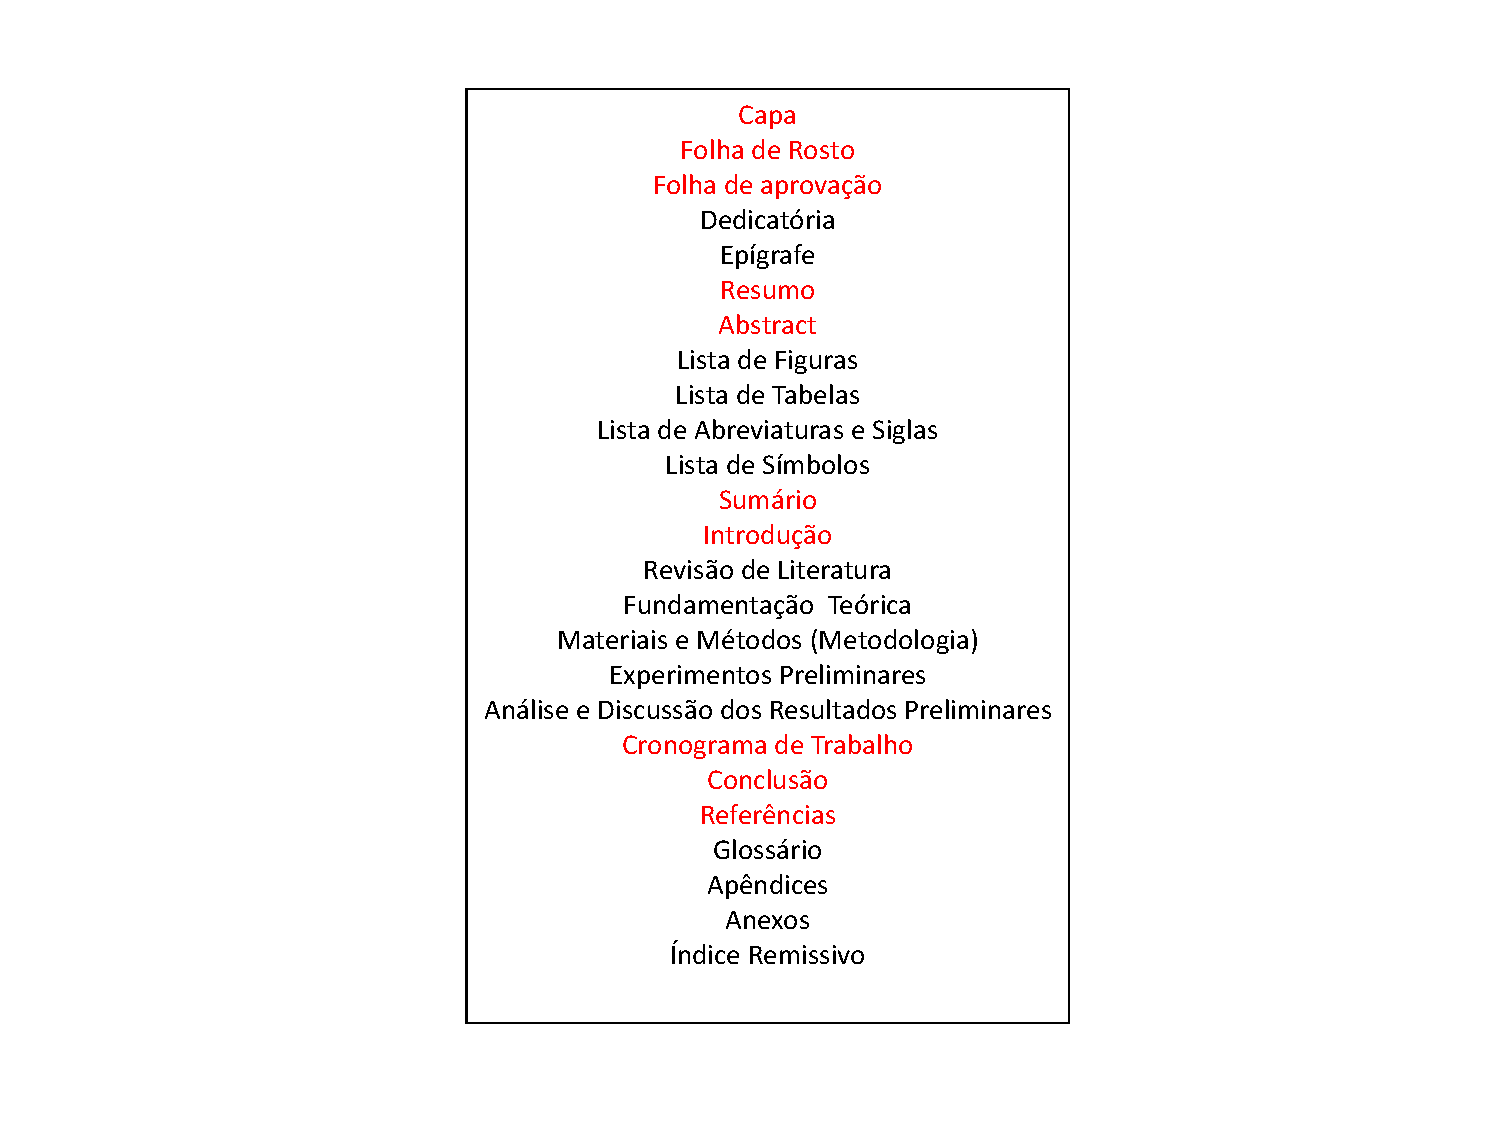
\includegraphics[width=0.5\textwidth]{./04-figuras/prjQualif-TeseDT_DissMT}
	%\fonte{\citeonline{CELSO2012}}
	\label{fig:prjQualif-TeseDT_DissMT}
\end{figure}


Já a \autoref{fig:teseDT_DissMT} apresenta uma estrutura para uma tese de doutorado ou dissertação de mestrado, conforme a norma \citeonline{NBR14724:2011}.

Cabe ressaltar que, em todas as figuras, os elementos obrigatórios estão destacados em vermelho, os demais são opcionais.


\begin{figure}[!h]
	\centering
	\caption{Estrutura sugerida de uma Tese de Doutorado ou Dissertação de Mestrado}
	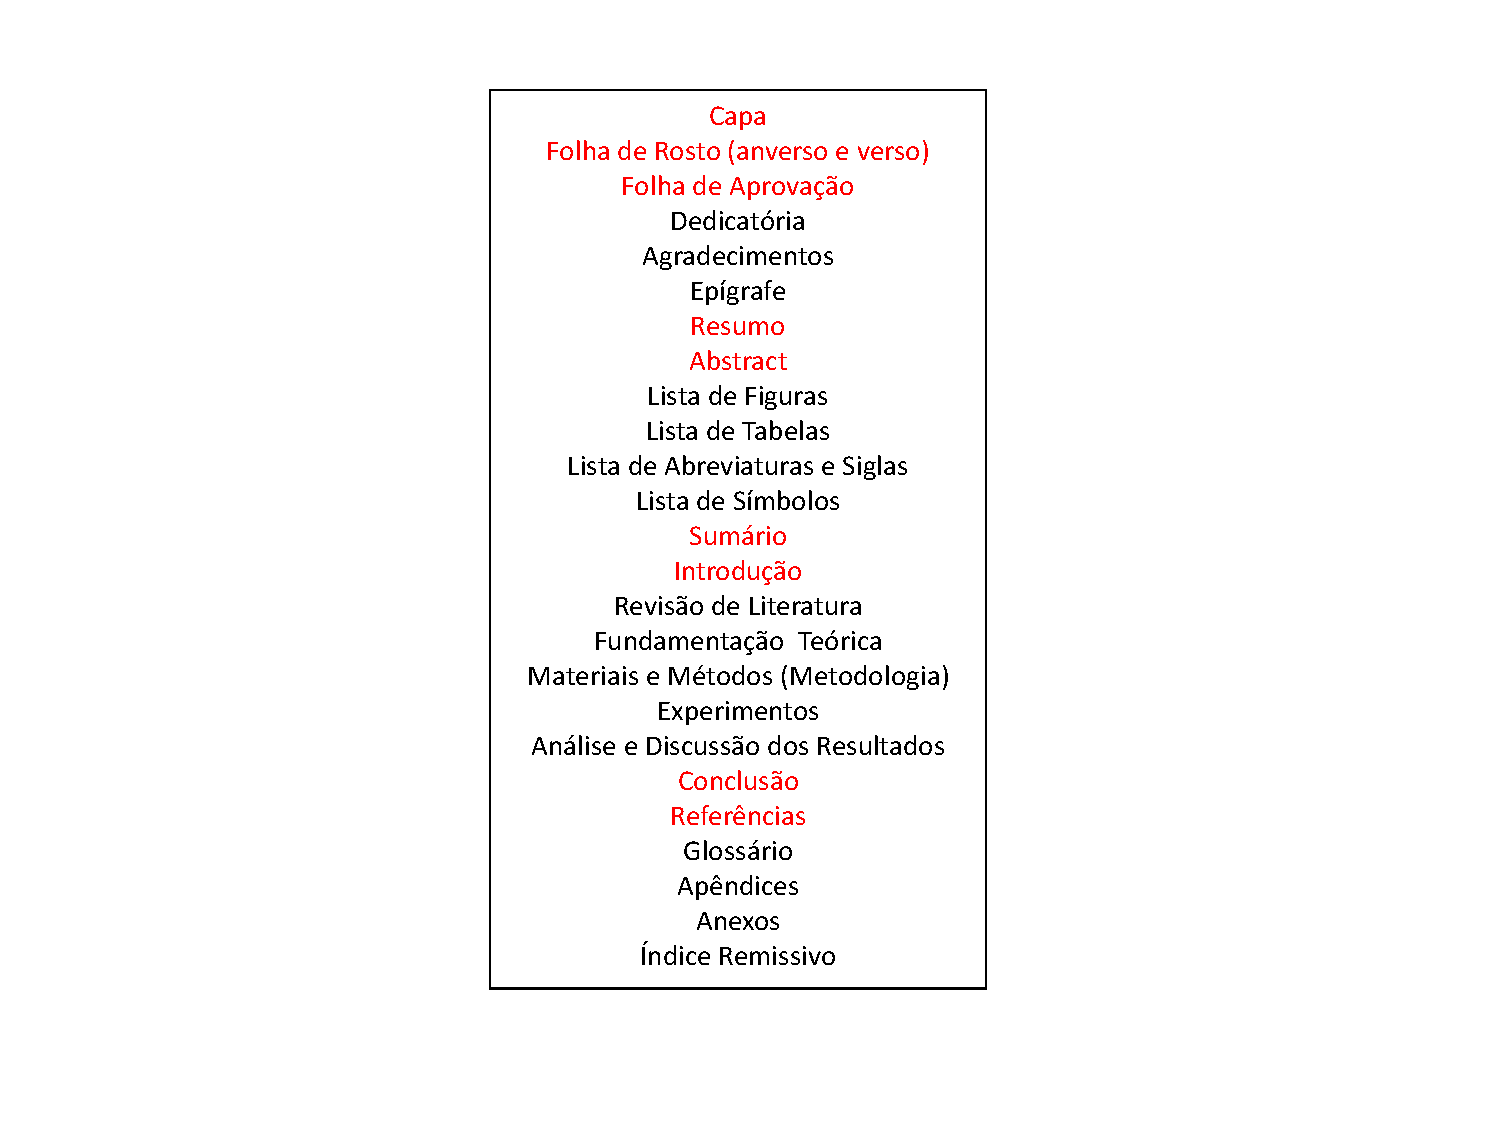
\includegraphics[width=0.5\textwidth]{./04-figuras/teseDT_DissMT}
	%\fonte{\citeonline{CELSO2012}}
	\label{fig:teseDT_DissMT}
\end{figure}


Observe que a estrutura de um projeto de qualificação é muito similar à da tese ou dissertação. A única diferença existente é que num projeto de qualificação o autor certamente terá, via de regra, apenas resultados parciais e preliminares. Além disso, estando o trabalho ainda em andamento, há que se apresentar um cronograma de trabalho que evidencie que o mesmo poderá ser concluído dentro dos prazos estabelecidos pelo programa.


Por fim, como foi dito, este  \emph{template} pode ser utilizado para outros trabalhos acadêmicos. Neste caso, a \autoref{fig:prjPesqAdmissao} apresenta uma sugestão de projeto de pesquisa a ser submetido ao programa para fins de admissão ao mesmo, conforme a norma \citeonline{NBR15287:2005}.

\begin{figure}[!htb]
	\centering
	\caption{Estrutura sugerida de um projeto de pesquisa para admissão ao PPGMMC}
	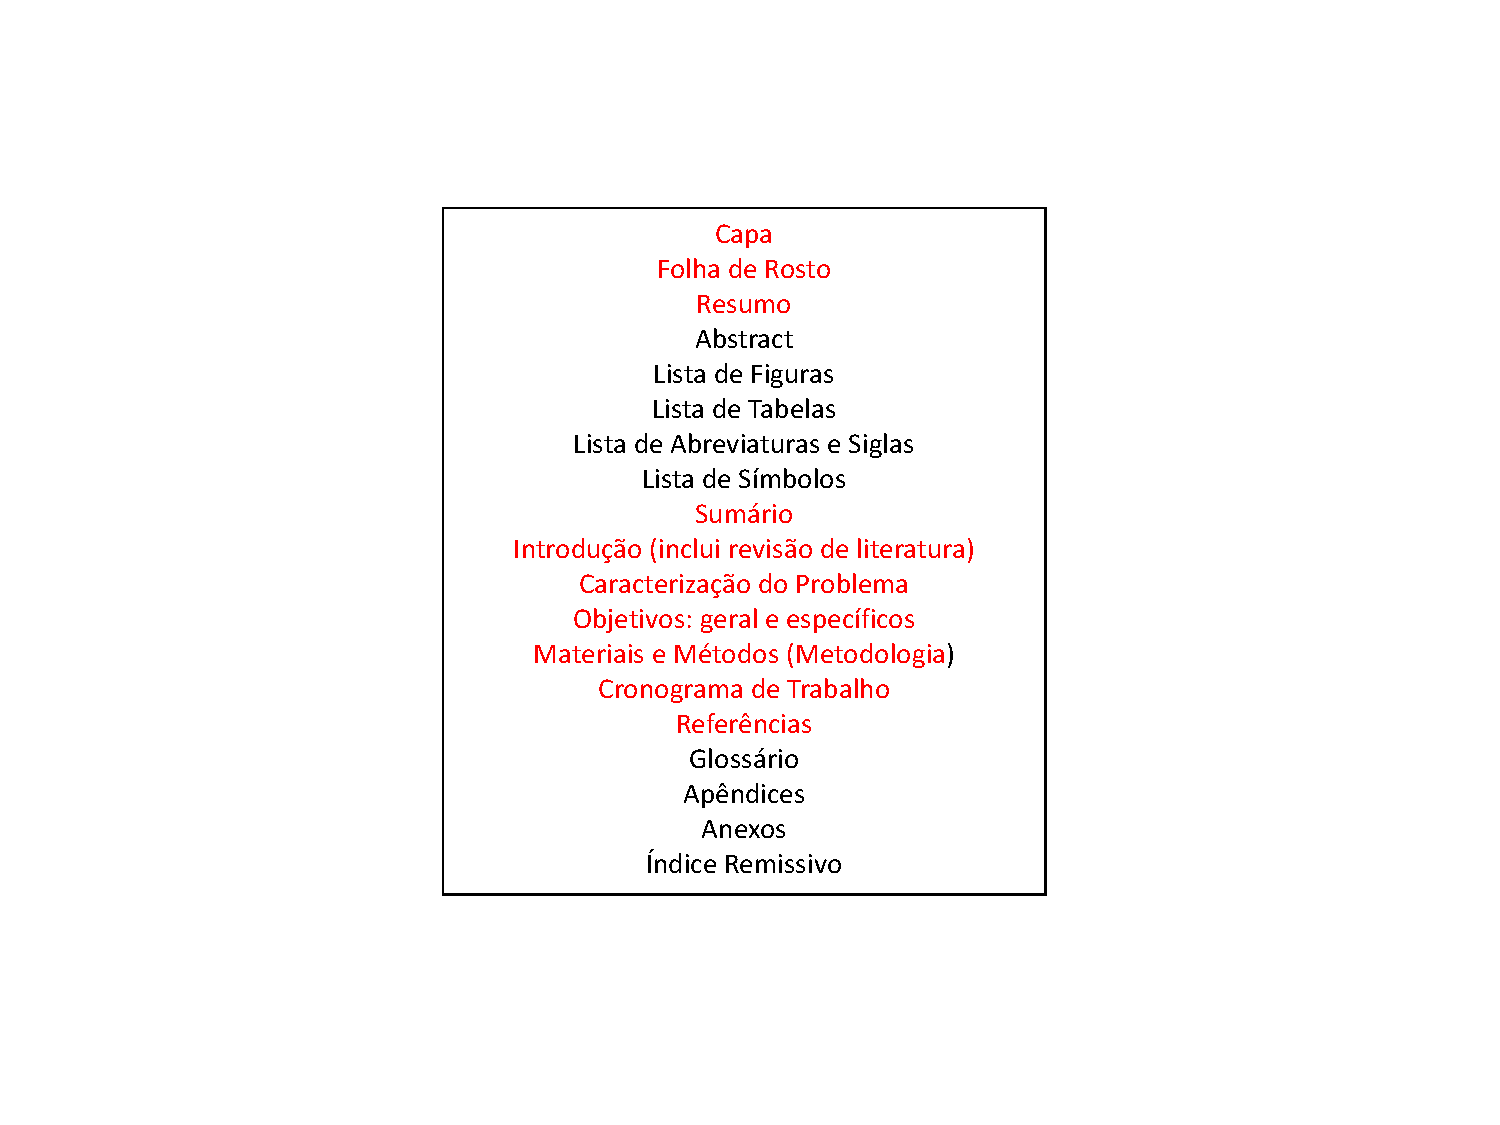
\includegraphics[width=0.6\textwidth]{./04-figuras/prjPesqAdmissao}
	%\fonte{\citeonline{CELSO2012}}
	\label{fig:prjPesqAdmissao}
\end{figure}

Você deverá editar o arquivo principal {\ttfamily meuTrabalhoAcademico.tex} para fazer os ajustes necessários, reiterando que as estruturas apresentadas são mera sugestão. 

A inclusão de reticências (\ldots) no texto deverá ser feita através de um comando especial denominado \verb|\ldots| \cite{LaTeX2014}. Assim esse comando deverá ser utilizado ao invés da digitação de três pontos.

Para melhor entendimento do uso do estilo de formatação, aconselha-se que o potencial usuário analise os comandos existentes no arquivo {\ttfamily main.tex} e os resultados obtidos no arquivo {\ttfamily main.pdf} depois do processamento pelo software \LaTeX{} + \textsc{Bib}\TeX{} \cite{LaTeX2014,BibTeX2014}.
Recomenda-se a consulta ao material de referência do software para a sua correta utilização \cite{Lamport1986,Buerger1989,Kopka2003,Mittelbach2004}.

Finalmente, este modelo apresenta um arquivo {\ttfamily makefile} para agilizar a compilação do documento \LaTeX{} e do \textsc{Bib}\TeX{}. portanto, para gerar o documento final no formato PDF, basta apenas executar o comando {\ttfamily make all} no linux. Para limpar os arquivos temporários, basta digitar o comando {\ttfamily make clean}.

O estilo de documento utilizado é o {\ttfamily abntex2}.
Através desse estilo a constituição do documento torna-se facilitada, uma vez que o mesmo possui comandos especiais para auxiliar a distribuição/definição das diversas partes constituintes do projeto.
Esse estilo é baseado nas normas da ABNT\index{ABNT}.

Maiores detalhes relacionados aos comandos existentes no estilo poderão ser adquiridos através da documentação disponível no site \href{https://code.google.com/p/abntex2/}{https://code.google.com/p/abntex2/} \cite{abnTeX22014b}.

Uma das principais vantagens do uso do estilo de formatação para \LaTeX{}  é a formatação \textit{automática} dos elementos que compõem um documento acadêmico, tais como capa, folha de rosto, dedicatória, agradecimentos, epígrafe, resumo, abstract, listas de figuras, tabelas, siglas e símbolos, sumário, capítulos, referências, etc.


% -----------------------------------------------------------------------------
% Novo apêndice
% -----------------------------------------------------------------------------

\chapter{Sobre as ilustrações}
\label{chap:apSobreIlust}

A seguir ilustra-se a forma de incluir ilustrações no corpo do texto. Pela norma figuras, tabelas, quadros, equações, quadros, algoritmos, diagrama, etc. são tipos específicos de ilustrações. As ilustrações (pelo menos alguns tipos específicos) serão indexadas automática em suas respectivas listas.

A numeração sequencial de figuras, tabelas e equações ocorre de modo automático.

Referências cruzadas são obtidas através dos comandos \verb|\label{}| e \verb|\ref{}|. Por exemplo, não é necessário saber que o número de certo capítulo é \ref{chap:fundamentacaoTeorica} para colocar o seu número no texto. Alternativamente se pode usar desta forma: \autoref{chap:fundamentacaoTeorica}. Isto facilita muito a inserção, remoção ou relocação de elementos numerados no texto (fato corriqueiro na escrita e correção de um documento acadêmico) sem a necessidade de renumerá-los todos.



\section{Figuras}
\label{sec:figuras}

Abaixo é apresentado um exemplo de figura.

A \autoref{fig:kdtree} aparece automaticamente na lista de figuras.

Para uso avançado de imagens no \LaTeX{}, recomenda-se a consulta de literatura especializada \cite{Goossens2007}.

\begin{figure}[!htb]
	\centering
	\caption{Exemplo da estrutura de uma árvore KD}
	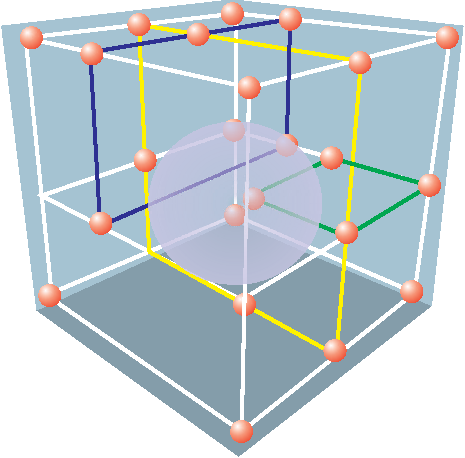
\includegraphics[width=0.5\textwidth]{./04-figuras/figkdtree}
	\fonte{\citeonline{Souza2012}}
	\label{fig:kdtree}
\end{figure}



\section{Quadros e tabelas}
\label{sec:tabelas}

Também é apresentado o exemplo do \autoref{qua:comparabd} e da \autoref{tab:testes}, que aparece automaticamente na lista de quadros e tabelas.

Informações sobre a construção de tabelas no \LaTeX{} podem ser encontradas na literatura especializada \cite{Lamport1986,Buerger1989,Kopka2003,Mittelbach2004}.

\begin{quadro}[!htb]
    \centering
    \caption{Hierarquia de restrições das questões.\label{qua:comparabd}}
    \begin{tabular}{|p{7cm}|p{7cm}|}
        \hline
        \textbf{BD Relacionais} & \textbf{BD Orientados a Objetos} \\
        \hline
        Os dados são passivos, ou seja, certas operações limitadas podem ser automaticamente acionadas quando os dados são usados. Os dados são ativos, ou seja, as solicitações fazem com que os objetos executem seus métodos. & Os processos que usam dados mudam constantemente. \\
        \hline
    \end{tabular}
    \fonte{\citeonline{Carvalho2001}}
\end{quadro}


Muitos confundem, mas existem diferenças entre tabelas e quadros.

Um quadro é formado por linhas horizontais e verticais, sendo, portanto ``fechado''. Você deverá utilizar um quadro quando o conteúdo é majoritariamente não-numérico. O número do quadro e o título vem acima do quadro, e a fonte, deve vir abaixo.

Uma tabela é formada apenas por linhas verticais, sendo, portanto ``aberta''. Você deverá utilizar uma tabela quando o conteúdo é majoritariamente numérico. O número da tabela e o título vem acima da tabela, e a fonte, deve vir abaixo, tal como no quadro.

Exemplo de tabela:

\begin{table}[!htb]
    \centering
    \caption[Resultado dos testes]{Resultado dos testes.
    \label{tab:testes}}
    \begin{tabular}{rrrrr}
        \toprule
            & Valores 1 & Valores 2 & Valores 3 & Valores 4 \\
        \midrule
            Caso 1 & 0,86 & 0,77 & 0,81 & 163 \\
            Caso 2 & 0,19 & 0,74 & 0,25 & 180 \\
            Caso 3 & 1,00 & 1,00 & 1,00 & 170 \\
        \bottomrule
    \end{tabular}
\end{table}




\section{Equações}
\label{sec:equacoes}

A transformada de Laplace é dada na \autoref{eq:laplace}, enquanto a Eq. \ref{eq:dft} apresenta a formulação da transformada discreta de Fourier bidimensional\footnote{Deve-se reparar na formatação esteticamente perfeita destas equações.}. Observe que utilizamos propositalmente duas formas distintas para referenciar as equações.

\begin{equation}
	X(s) = \int\limits_{t = -\infty}^{\infty} x(t) \, \text{e}^{-st} \, dt
	\label{eq:laplace}
\end{equation}

\begin{equation}
	F(u, v) = \sum_{m = 0}^{M - 1} \sum_{n = 0}^{N - 1} f(m, n) \exp \left[ -j 2 \pi \left( \frac{u m}{M} + \frac{v n}{N} \right) \right]
	\label{eq:dft}
\end{equation}



\section{Algoritmos}\label{sec:algoritmos}

Os algoritmos devem ser feitos segundo o modelo abaixo. Para isso, utilizar o pacote {\ttfamily algorithm2e} no início do arquivo principal como neste exemplo.
\\
\\

\begin{algorithm}
    \caption{Algoritmo para remoção aleatória de vértices}
    \KwIn{o número $n$ de vértices a remover, grafo original $G(V, E)$}
    \KwOut{grafo reduzido $G'(V,E)$}
    $removidos \leftarrow 0$ \\
    \While {removidos $<$ n } {
        $v \leftarrow$ Random$(1, ..., k) \in V$ \\
            \For {$u \in adjacentes(v)$} {
                remove aresta (u, v)\\
                $removidos \leftarrow removidos + 1$\\
            }
            \If {há  componentes desconectados} {
                remove os componentes desconectados\\
            }
        }
\end{algorithm}



% -----------------------------------------------------------------------------
% Novo apêndice
% -----------------------------------------------------------------------------

\chapter{Sobre as listas}
\label{chap:apSobreLista}


Para construir listas de "\textit{bullets}"{} ou listas enumeradas, inclusive listas aninhadas, é utilizado o pacote \verb|paralist|.

O exemplo a seguir ilustra duas listas não numeradas aninhadas, utilizando o ambiente \verb|\compactitem|. Observe a indentação, bem como a mudança automática do tipo de "\textit{bullet}"{} nas listas aninhadas.



\begin{compactitem}
	\item item não numerado 1
	\item item não numerado 2
	\begin{compactitem}
		\item subitem não numerado 1
		\item subitem não numerado 2
		\item subitem não numerado 3
	\end{compactitem}
	\item item não numerado 3
\end{compactitem}


Por outro lado, o exemplo a seguir ilustra duas listas numeradas aninhadas, utilizando o ambiente \verb|\compactenum|. Observe a numeração progressiva e indentação das listas aninhadas.


\begin{compactenum}
	\item item numerado 1
	\item item numerado 2
	\begin{compactenum}
		\item subitem numerado 1
		\item subitem numerado 2
		\item subitem numerado 3
	\end{compactenum}
	\item item numerado 3
\end{compactenum}

Cabe ressaltar que os ambientes \verb|\itemize| e \verb|\enumerate| podem ser utilizados alternativamente. No entanto, durante a compilação pdflatex são apresentados erros associados a estes ambientes, porém o pdf é gerado corretamente. Trata-se de um "\textit{bug}"{} que ainda não conseguimos resolver. Caso conheça a solução, por favor, comunique-nos para que possamos incluí-la numa futura atualização deste modelo.


% -----------------------------------------------------------------------------
% Novo apêndice
% -----------------------------------------------------------------------------

\chapter{Sobre citações e chamadas de referências}
\label{chap:apSobreCita}


Citações são trechos transcritos ou informações retiradas das publicações consultadas para a realização do trabalho.
As citações são utilizadas no texto com o propósito de esclarecer, completar, embasar ou corroborar as ideias do autor.

Todas as publicações consultadas e efetivamente utilizadas (por meio de citações) devem ser listadas, obrigatoriamente, nas referências bibliográficas, de forma a preservar os direitos autorais e intelectuais.

A norma ABNT NBR:10520-2002 classifica as citações em: citações livres e citações literais.



\section{Citações livres}
\label{sec:citacoesLivres}


Nas citações livres, reproduzem-se as ideias e informações de um autor, sem, entretanto, ``copiar letra por letra'' o texto do autor. Sendo assim, não há muito a dizer sobre como fazer citações livres, exceto que há que se tomar o devido cuidado com o "recortar e colar e modificar"{} para que não se caracterize plágio.

Quanto à chamada da referência, ela pode ser feita de duas maneiras distintas, conforme o nome do(s) autor(es) façam parte do seu texto ou não. Os exemplos a seguir ilustram estas duas possibilidades.

Enquanto \citeonline{Maturana2003} defendem uma epistemologia baseada na biologia. Para os autores, é necessário rever \ldots.

Por outro lado, \citeonline{Barbosa2004} contra-argumenta afirmando que \ldots.

Acima, as chamadas de referências foram feitas com o comando \verb|\citeonline{chave}|, que produzirá a formatação correta, conforme a norma ABNT.

 Observe que em ambos os casos anteriores, a frase fica incompleta e incompreensível caso as palavras "Maturana e Varela"{} e "Barbosa et al."{} não sejam "pronunciadas"{}. Ou seja, os nomes dos autores fazem parte da frase. Neste caso, a formatação automática da chamada de referência coloca os nomes dos autores seguido, entre parêntesis pelo ano de publicação da obra referenciada. Isso apenas no caso em que se usa o esquema autor-ano, que é \textit{padrão} neste modelo \LaTeX{}.

A segunda maneira de fazer uma chamada de referência deve ser utilizada quando se quer evitar uma interrupção na sequência do texto, o que poderia, eventualmente, prejudicar a leitura.

Assim, a citação livre é feita e imediatamente após a obra referenciada deve ser colocada entre parênteses. Porém, neste caso específico, o nome do autor deve vir em caixa alta, seguido do ano da publicação, como nos exemplos a seguir.

Há defensores da epistemologia baseada na biologia que argumentam em favor da necessidade de \ldots \cite{Maturana2003}.

Por outro lado, há os que contra-argumentam afirmando que \ldots  \cite{Barbosa2004}.

Nos dois casos imediatamente acima a chamada de referência deve ser feita com o comando \verb|\cite{chave}|, que produzirá a formatação correta, conforme a norma ABNT.

Observe que o estilo de redação das frases teve que ser modificado para torná-las compreensíveis sem a menção explícita dos nomes dos autores. Estes agora não são parte integrante da frase, ficam entre parêntesis. Neste caso, a formatação automática da chamada de referência coloca, entre parêntesis, os nomes dos autores seguido pelo ano de publicação da obra referenciada. Novamente, apenas no caso em que se usa o esquema autor-ano, que é \textit{padrão} neste modelo \LaTeX{}.

Por fim, cabe chamar a atenção para o detalhe do termo \textit{et al.} que deve ser utilizado quando o trabalho citado possui mais de três autores. Esse recurso é automatizado pelo estilo {\ttfamily abntex2}. Caso não haja desejo em abreviar o nome dos demais autores através do termo \textit{et al.}, deve-se incluir a opção {\ttfamily abnt-no-etal-label}. 



\section{Citações literais}
\label{sec:citacoesLiterais}

Nas citações literais, reproduzem-se as ideias e informações de um autor, exatamente como este a expressou, ou seja, faz-se uma ``cópia letra por letra'' do texto do autor. Sendo assim, obviamente, a obra citada deve ser referenciada, sob pena de se caracterizar plágio.

Quanto à chamada da referência, ela pode ser feita de qualquer das duas maneiras mencionadas na \autoref{sec:citacoesLivres}, conforme o nome do(s) autor(es) façam parte do seu texto ou não.

Há duas maneiras distintas de se fazer uma citação literal, conforme o trecho citado seja longo ou curto.

Quando o trecho citado é longo (4 ou mais linhas) deve-se usar um parágrafo específico para a citação, na forma de um texto recuado (4 cm da margem esquerda), com tamanho de letra menor do aquela utilizada no texto e espaçamento entrelinhas simples. Veja o exemplo abaixo.

\begin{citacao}
	Desse modo, opera-se uma ruptura decisiva entre a reflexividade filosófica, isto é a possibilidade do sujeito de pensar e de refletir, e a objetividade científica. 	Encontramo-nos num ponto em que o conhecimento científico está sem consciência. Sem consciência moral, sem consciência reflexiva e também subjetiva. Cada vez mais o desenvolvimento extraordinário do conhecimento científico vai tornar menos praticável a própria possibilidade de reflexão do sujeito sobre a sua pesquisa \cite[p.~28]{Silva2000}.
\end{citacao}

Para se criar o efeito demonstrado na citação anterior, deve-se utilizar o comando:

\begin{verbatim}
\begin{citacao}
<citacao>
\end{citacao}
\end{verbatim}

Acima, para a chamada da referência o comando \verb|\cite[p.~28]{Silva2000}| foi utilizado, visto que os nomes dos autores não são parte do trecho citado.

Observe ainda que foi indicado o número da página da obra citada que contém o trecho citado. A localização precisa do trecho citado deve ser indicada sempre, exceto para artigos científicos (tipicamente com poucas páginas, o que geralmente não é o caso de artigos de revisão de literatura) e outros documentos com "poucas"{} páginas.

Alternativamente, é possível construir uma frase que contenha os autores, e irá encaminhar (por assim dizer) a citação literal. Assim sendo, note que pode após a citação literal não mais aparece o nome dos autores, visto que já se encontra no texto. Veja o exemplo seguinte.

No entanto, \citeonline[p.~33]{Silva2000}, ao fazerem as suas críticas à ciência moderna, afirmam:

\begin{citacao}
	Mas o curioso é que o conhecimento científico que descobriu os meios realmente extraordinários para, por exemplo, ver aquilo que se passa no nosso sol, para tentar conceber a estrutura das estrelas extremamente distantes, e até mesmo para tentar pesar o universo, o que é algo de extrema utilidade, o conhecimento científico que multiplicou seus meios de observação e de concepção do universo, dos objetos, está completamente cego, se quiser considerar-se apenas a si próprio!
\end{citacao}


Já quando o trecho citado é curto (3 ou menos linhas) ele deve inserido diretamente no texto entre aspas. Veja os dois exemplos seguintes, cada qual utilizando uma forma de chamada de referência.

A epistemologia baseada na biologia parte do princípio de que ``assumo que não posso fazer referência a entidades independentes de mim para construir meu explicar'' \cite[p.~35]{Maturana2003}.

A epistemologia baseada na biologia de \citeonline[p.~35]{Maturana2003} parte do princípio de que ``assumo que não posso fazer referência a entidades independentes de mim para construir meu explicar''.

Finalmente, e isto vale para citações curtas ou longas, caso seja necessário inserir ou suprimir (modificar de modo geral) qualquer palavra ou frase no trecho citado literalmente, qualquer que seja a finalidade, isto deve ser feito colocando sua intervenção entre colchetes retos e deve ser indicado explicitamente ao final da citação. Veja o exemplo seguinte.

A epistemologia baseada na biologia parte do princípio de que ``assumo que não posso fazer referencia [\textit{sic}] a \underline{entidades independentes} de mim [realidade objetiva] para construir meu explicar'' \cite[p.~35, comentários e grifo nosso]{Maturana2003}.



\section{Mais detalhes sobre as chamadas de referências}
\label{sec:referUtilizadas}


A seguir há mais exemplos dos comandos para as chamadas de referências e o resultado produzido.


\citeonline{Maturana2003} \ \ \  \verb|\citeonline{Maturana2003}|\\
\citeonline{Barbosa2004} \ \ \   \verb|\citeonline{Barbosa2004}|\\
\cite[p.~28]{Silva2000} \ \ \  \verb|\cite[p.~28]{Silva2000}|\\
\citeonline[p.~33]{Silva2000} \ \ \   \verb|\citeonline[p.~33]{v}|\\
\cite[p.~35]{Maturana2003} \ \ \   \verb|\cite[p.~35]{Maturana2003}|\\
\citeonline[p.~35]{Maturana2003} \ \ \   \verb|\citeonline[p.~35]{Maturana2003}|\\
\cite{Barbosa2004,Maturana2003} \ \ \   \verb|\cite{Barbosa2004,Maturana2003}|\\


Há que se tomar bastante cuidado com referências cujos autores têm nomes compostos, tipo João de Souza Júnior ou Antônio José da Silva Filho. Para que a formatação seja correta, os nomes dos autores no arquivo {\ttfamily .bib} deverá ser cadastrado de uma forma específica. Para maiores detalhes, veja o \autopageref{chap:anexoB} \footnote{O texto do anexo é de inteira responsabilidade do autor devidamente referenciado.}.

Os exemplos abaixo ilustram a formatação correta.


\cite[p.~28]{vanGELDER1998} \ \ \ \ \  \verb|\cite[p.~28]{vanGELDER1998}|\\
\citeonline[p.~28]{vanGELDER1998} \ \ \ \ \  \verb|\citeonline[p.~28]{vanGELDER1998}|\\
\cite[p.~35]{Silva2013} \ \ \ \ \  \verb|\cite[p.~35]{Silva2013}|\\
\citeonline[p.~35]{Silva2013} \ \ \ \ \  \verb|\citeonline[p.~35]{Silva2013}|\\


Observe que, a despeito do que está dito no \autoref{chap:anexoB}, ainda há falhas na formatação ABNT de nomes tipo \verb|van Gelder| quando utilizados em chamadas de referências que fazem parte do texto (\textit{e.g.}, \verb|\citeonline{vanGELDER1998}| que deveria produzir \verb|van Gelder (1998)|). Este problema pode ser contornado facilmente, simplesmente evitando o uso dessa forma de chamada de referência, preferindo sempre nestes casos, o uso da forma \textit{e.g.}, \verb|\cite{vanGELDER1998}| que será formatada corretamente, produzindo \verb|(van GELDER, 1998)|.

Observe ainda o caso em que é feita duas citações juntas \cite{Santos2003, Neubert2001, Silva2013} e como citar endereços Web \cite{IRL2014}. 


% -----------------------------------------------------------------------------
% Novo apêndice
% -----------------------------------------------------------------------------

\chapter{Sobre as referências bibliográficas}
\label{chap:apSobreRefer}

A bibliografia é feita no padrão \textsc{Bib}\TeX{}. As referências são colocadas em um arquivo separado. Os elementos de cada item bibliográfico que devem constar nas referências  bibliográficas são apresentados a seguir. Tais referências bibliográficas devem seguir a norma \citeonline{NBR6023:2002} da ABNT\footnote{As normas técnicas da ABNT não são gratuitas.}.



\section{Entradas de referências}
\label{sec:entradasRefs}

Entradas são objetos de citação bibliográficas. Dito de outra forma, são as categorias dos tipos de documentos e materiais componentes da bibliografia. A classe abn\TeX{} define as seguintes entradas:


\begin{verbatim}
@book
@inbook
@article
@phdthesis
@mastersthesis
@monography
@techreport
@manual
@proceedings
@inproceedings
@journalpart
@booklet
@patent
@unpublished
@misc
\end{verbatim}

Cada entrada é formatada pelo pacote \citeonline{abnTeX22014d} de uma forma específica. Algumas entradas foram introduzidas especificamente para atender à norma \citeonline{NBR6023:2002}, são elas: \verb|@monography|, \verb|@journalpart|,\verb|@patent|. As demais entradas são padrão \textsc{Bib}\TeX{}. Para maiores detalhes, refira-se a \citeonline{abnTeX22014d}, \citeonline{abnTeX22014b}, \citeonline{abnTeX22014c}.

A entrada \verb|@monography| é utilizada para cadastrar referências a trabalhos de conclusão de curso, monografias de cursos de especialização (pós-graduação \textit{lato sensu}), e outros trabalhos monográficos, exceto dissertação de mestrado e tese de doutorado. Eu particularmente, não considero que a formatação deste tipo de entrada está adequado. Para um trabalho de conclusão de curso (TCC) de curso de graduação, que deveria ser formatado como "[\ldots] Trabalho de Conclusão de Curso (Bacharelado em Engenharia de Computação) [\ldots]"{}; no entanto o uso de \verb|@monography| irá produzir "[\ldots] Monografia (Bacharelado em Engenharia de Computação) [\ldots]"{}. A própria  \citeonline{NBR6023:2002}, na seção 8.11.4, apresenta um exemplo com a formatação diferente daquela proporcionada por \citeonline{abnTeX22014d}.

A entrada \verb|@journalpart| é utilizada, conforme diz o manual \cite{abnTeX22014d}, para cadastrar referências e formatar partes de periódicos. Não fica claro o que se quer dizer com partes de journal. Em alguns casos, tais partes são artigos - e portanto, deveriam ser registradas como \verb|@article| - noutros casos, parece serem matérias ou textos em revistas ou jornais (não científicos). Salvo melhor juízo, me parece que esta entrada deve ser utilizada apenas neste último contexto.

A entrada \verb|@patent| é utilizada, obviamente, para cadastrar referências a patentes.

Na \autoref{chap:softApoio} recomendamos o uso de algum sistema para o gerenciamento de referências bibliográficas (\textit{e.g.}, Mendeley, JabRef, Zotero, etc.), Os próprios \textit{publishers} frequentemente disponibilizam, juntamente com o documento (artigo, livro, etc.) o arquivo {\ttfamily .bib} que contém a referência  \textsc{Bib}\TeX{} daquele documento. Assim, o \textit{software} de apoio facilita bastante a manutenção de coleções de referências bibliográficas.

Todavia, o fato é que a normalização de referências conforme a norma \citeonline{NBR6023:2002} requer que muitos dos campos do \textsc{Bib}\TeX{} sejam adaptados. Sendo mais explícito, ao baixar um arquivo {\ttfamily .bib} de um trabalho, principalmente ser for internacional, e inserí-lo "\textit{as is}"{} em suas referências, há grande chance dessa referência ser formatada de modo errado, no que concerne à norma \citeonline{NBR6023:2002}. Isso é especialmente válido em alguns tipos de documentos de largo uso no meio acadêmico afim às áreas de Ciências Exatas, da Terra e Engenharias.

Diante disso, para evitar erros de formatação, o correto é após baixar o arquivo {\ttfamily .bib} de um trabalho, editá-lo com um editor ASCII (usando codificação UTF8), para verificar se os campos descritores que o \textit{publishers} original utilizou são aqueles requeridos pela norma ABNT.

Neste contexto, e para esta finalidade, nas seções seguintes é apresentado uma série de exemplos, quase todos, utilizados como exemplos na própria norma \citeonline{NBR6023:2002}. Para detalhes dos campos utilizados confira o arquivo {\ttfamily myRefs.bib}. Deve-se estar atento para o fato de que o uso de um sistema de gerenciamento de referências para abrir e/ou editar o arquivo {\ttfamily myRefs.bib}, pode ocultar campos utilizados pela norma ABNT e, por outro lado, exibir campos não utilizados por ela. Ou seja, o aplicativo deve ser configurado adequadamente para exibir \textbf{todos os campos}, mesmo os opcionais.



\section{Notas de rodapé}
\label{sec:notasRodape}


A norma \citeonline{NBR10520:2002}, em sua seção \textbf{7 Notas de rodapé}, classifica as notas de rodapé em duas categorias: notas explicativas\footnote{é o tipo mais comum de notas que destacam, explicam e/ou complementam o que foi dito no corpo do texto, como esta nota de rodapé, por exemplo.} e notas de referências. Já as notas de referências, como o próprio nome ja indica, são utilizadas para colocar referências e/ou chamadas de referências sob certas condições.



\subsection{Referências em notas de rodapé: uso do \textit{apud}}
\label{subsec:refRodape}


Para citar uma referência que, por sua vez, foi citada por outra referência, por exemplo no caso Fulano (2000 apud CICLANO, 2002, p. 57). pode-se usar as macros \verb|\apud| ou \verb|\apudonline|, equivalentes aos casos \verb|\cite| e \verb|\citeonline|, respectivamente.

A título de exemplo, veja o que foi digitado: 

\begin{verbatim}
O modelo canônico de documentos formatados conforme as norma da ABNT
\apud[p.~2]{abnTeX22014a}{abnTeX22014c} oferece [\ldots].
\end{verbatim}

e a saída formatada produzida:

O modelo canônico de documentos formatados conforme as norma da ABNT \apud[p.~2]{abnTeX22014a}{abnTeX22014c} oferece [\ldots].

Por outro lado, utilizando o \verb|apudonline|, o texto digitado:

\begin{verbatim}
Assim, \apudonline[p.~2]{abnTeX22014a}{abnTeX22014c} apresentam seu
modelo canônico de documentos formatados conforme as norma da ABNT [\ldots].
\end{verbatim}

produzirá a saída assim formatada:

Assim, \apudonline[p.~2]{abnTeX22014a}{abnTeX22014c} apresentam seu modelo canônico de documentos formatados conforme as norma da ABNT [\ldots].


Nos casos anteriores, ambas as referências - tanto \verb|{abnTeX22014a}| quanto \verb|{abnTeX22014c}|, aparecerão na lista de referências, exceto se alguma delas for definida como entrada \texttt{@hidden}. Mais explicitamente, se você não quiser que uma entrada apareça na lista de referências, você deve defini-la como do tipo \texttt{@hidden} em seu arquivo \textsc{Bib}\TeX{}.

Neste caso, a obra \verb|{abnTeX22014a}| não foi consultada, portanto, não deve estar na lista de referências e deverá ser referenciada como nota de rodapé. No caso em questão, deve-se cadastrar a entrada de \textit{label} \verb|{abnTeX22014a}| como \texttt{@hidden}.

Para ver como referenciá-la numa nota de rodapé, veja a seção seguinte.



\subsection{Referências em notas de rodapé: uso do comando \textit{footciteref}}
\label{subsec:refFootCite}

O posicionamento de referência em notas de rodapé é às vezes uma necessidade. No caso específico de citação de citação - que requer o uso do \textit{apud} - a obra indiretamente citada - \verb|{abnTeX22014a}| - deverá ter sua referência completa colocada em uma nota de rodapé, como prescreve a seção \textbf{7.1 Notas de referência} da norma \citeonline{NBR10520:2002}. Para tanto usa-se o comando \verb|\footciteref{abnTeX22014a}|.

No caso do exemplo mencionado na seção anterior, o uso de

\begin{verbatim}
O modelo canônico de documentos formatados conforme as norma da ABNT
\apud[p.~2]{abnTeX22014a}{abnTeX22014c} \footciteref{abnTeX22014a}
oferece [\ldots].
\end{verbatim}

irá produzir a chamada de referência indireta, bem como irá colocar a referência completa da obra citada indiretamente em nota de rodapé. Senão vejamos:

O modelo canônico de documentos formatados conforme as norma da ABNT \apud[p.~2]{abnTeX22014a}{abnTeX22014c} \footciteref{abnTeX22014a} oferece [\ldots].

Observe que, neste caso, o comando \verb|\footciteref{abnTeX22014a}| criou a nota de rodapé, porém não colocou a referência completa nele. Trata-se, aparentemente, de uma falha na implementação deste comando, que é específico do pacote \texttt{abntex2cite}, no qual seu uso \textbf{exige} que a referência seja visível (não funciona caso a entrada seja \texttt{@hidden}). Isso se contrapõe à própria norma, como observado por  \citeonline[p.~7]{abnTeX22014c}.

Como solução parcial, até que tal comando seja revisado, propomos que se utilize uma  nota de rodapé usual, mediante o comando  \verb|\footnote{referencia elaborada manualmente}|.

No caso anteriormente mencionado, a digitação de:

\begin{verbatim}
O modelo canônico de documentos formatados conforme as norma da ABNT
\apud[p.~2]{abnTeX22014a}{abnTeX22014c} \footnote{ABNTEX2; ARA\'UJO,
L. C. \textbf{A classe abntex2}: Documentos técnicos e científicos
brasileiros compatíveis com as normas abnt. [S.l.], 2014. 46 p.
Disponível em: \href{https://code.google.com/p/abntex2/wiki/Download?tm=2}
{http://abntex2.googlecode.com/}. Acesso em: 12 de setembro de 2014.}
oferece [\ldots].
\end{verbatim}

irá produzir o texto a seguir incluindo uma nota de rodapé, contendo a referência completa para a entrada \verb|{abnTeX22014a}| (colocada como oculta), porém formatada manualmente. Senão vejamos:
\\
\\
O modelo canônico de documentos formatados conforme as norma da ABNT \apud[p.~2]{abnTeX22014a}{abnTeX22014c} \footnote{A referência original pode ser encontrada em \textcolor{blue}{ABNTEX2; ARA\'UJO, L. C. \textbf{A classe abntex2}: Documentos técnicos e científicos brasileiros	compatíveis com as normas abnt. [S.l.], 2014. 46 p. Disponível em: \href{https://code.google.com/p/abntex2/wiki/Download?tm=2}{http://abntex2.googlecode.com/}. Acesso em: 12 de setembro de 2014.}} oferece [\ldots].


Resolvido esta dificuldade do modelo, resta indicar que o \textit{hiperlink} aposto em \citeonline{abnTeX22014a} continuará funcionando, porém apontará para a página da capa do trabalho e não para uma referência real (pois esta referência não consta da lista de referências). Eventualmente isto poderia ser modificado para que apontasse para a nota de rodapé correspondente, no entanto, haveria que alterar mais profundamente o modelo, o que nos parece desnecessário no momento.



\subsection{Notas de referências: uso de idem, ibidem, opus citatus e outros}
\label{subsec:notasRefs}

Como indica o próprio nome, as notas de referências se prestam como recurso auxiliar para referenciação de bibliografia, e seu uso e aplicação são descritos na seção \textbf{7.1 Notas de referência} da norma \citeonline{NBR10520:2002}. 

Estes recursos se referem ao uso de certas expressões consagradas para facilitar a elaboração de referencias. São eles:

\begin{compactitem}
	\item idem = mesmo autor,
	\item ibidem = mesma obra,
	\item opus citatum = obra citada,
	\item locus citatum = no lugar citado,
	\item passim = aqui e alí,
	\item cf = confira,
	\item et sequentia = e sequência.
\end{compactitem}


Observe que estes recursos não se adequam para serem utilizados em listas de referências bibliográficas, nem tampouco no corpo do texto. Assim, devem ser utilizados apenas nas notas de referência posicionadas no rodapé \cite[p.~6]{abnTeX22014c}, quando se referem a uma referência já feita anteriormente no corpo do texto. Ademais, essas expressões fazem sentido apenas quando aplicadas a citações de uma única referência por vez. Enfim, trata-se mais de um recurso estilístico do que algo de primeira necessidade, pelo menos para o tipo de documento usualmente elaborados nas área de Ciências Exatas, da Terra e Engenharias.

Veja o uso desses tipos de expressões nos exemplos seguintes:


\Idem[p.~21]{abnTeX22014d}

\Ibidem[p.~7]{abnTeX22014c}

\opcit[p.~9]{abnTeX22014c}

\passim{abnTeX22014c}

\cfcite[p.~3]{abnTeX22014b}

\etseq[p.~6]{abnTeX22014c}



\section{Datas em referências}
\label{sec:datasBib}


Quando as chamadas de referências são feitas no modelo autor-ano, como é o caso deste modelo \LaTeX{}, é evidente que o autor e sobretudo o ano adquirem papel de destaque. No caso da data de publicação, esta deve sempre estar presente (é elemento essencial) e indicada em algarismos arábicos.

A norma ABNT não permite o uso de expressões do tipo "sem data"{} ("[s.d]") para indicar que não se sabe a data de publicação de certa referência bibliográfica. Assim sendo, quando a data não puder ser indicada precisamente, deve-se registrar uma data aproximada entre colchetes, conforme descrito a seguir:


[1971 ou 1972] \ \ \ \ \ um ano ou outro,

[1969?] \ \ \ \ \ ano provável,

[1973] \ \ \ \ \ ano certo, não indicada no item,

[entre 1906 e 1912] \ \ \ \ \ use intervalos menores de 20 anos,

[ca. 1960] \ \ \ \ \ \textit{circa} de ... ( data aproximada),

[197-] \ \ \ \ \ década certa,

[197-?] \ \ \ \ \ década provável,

[18--] \ \ \ \ \ século certo,

[18--?] \ \ \ \ \ século provável.


% -----------------------------------------------------------------------------
% Novo apêndice
% -----------------------------------------------------------------------------

\chapter{Exemplos de referencias normalizadas pela NBR 6023:2002}
\label{chap:apExemplosRefs}

Antes de mais nada, cabe dizer que as normas \citeonline{NBR6023:2002} - elaboração de referências e \citeonline{NBR10520:2002} - citações em documentos, não são (ou melhor, não devem ser) independentes uma da outra e, portanto, requerem uma boa dose de interpretação, como de resto é usual em se tratando de normas.

Estas normas tem várias lacunas e inconsistências, o que torna uma tarefa ingrata a construção de um modelo, tal como este, que atenda a todos os inúmeros requisitos de formatação da norma. A dificuldade não é apenas com o fato de ser necessário a inclusão de um sem número de novos atributos e comandos \LaTeX{}, mas, principalmente, por ser necessário dar uma interpretação dessas normas de modo a "sanar"{} suas inconsistências.

Dito isso, resta dizer que todo o esforço foi feito para que todos os tipos de referências sejam formatadas conforme estabelece a norma \citeonline{NBR6023:2002}, no entanto, é claro, que em alguns casos não foi logrado êxito. De fato, desconheço a existência de um modelo \LaTeX{} que formate todo tipo de referências com precisão, todos falham em algum aspecto, por menor que seja.

Dito isso, deve-se louvar o trabalho realizado pele equipe  \textsc{ABN}\TeX\textsc{2} na construção do pacote \texttt{abntex2cite}. Eles procuraram reproduzir com o máximo de fidedignidade, usando o \LaTeX, todos, ou quase todos, os exemplos apresentados nas normas. A eles, todo o crédito é devido. Que fique claro, porém, que em alguns poucos casos os autores não lograram pleno êxito. De fato, desconhecemos a existência de um modelo \LaTeX{} que formate todo tipo de referências com precisão, todos falham em algum aspecto, por menor que seja.

Neste apêndice, apresentamos o conjunto de exemplos de referências\footnote{A norma estabelece que seus exemplos tem caráter normativo, e não apenas ilustrativo.}, presentes na norma ABNT NBR 6023:2002 \cite{NBR6023:2002} - elaborado por  \citeonline{abnTeX22014d} no formato \textsc{Bib}\TeX{}. Este conjunto compõe o arquivo \verb|abntex2-doc-1.9.2.zip| disponibilizado na referência recém-citada. Este conjunto foi complementado com um pequeno conjunto de referências que elaboramos e utilizamos nos vários exemplos presentes principalmente nestes Apêndices, elas foram indicadas pela expressão "referência nossa"{} logo após a respectiva chamada de referência.

As referências apresentadas nas seções seguintes, foram agrupadas conforme os tipos de entrada que foram utilizados em seu cadastramento no \textsc{Bib}\TeX{}.

Em alguns pouquíssimos casos, pequenas correções absolutamente pontuais foram feitas no texto original do arquivo \verb|.bib|, em particular onde os próprios autores manifestavam alguma dúvida. Todas as notas de referências foram elaboradas pelos autores originais. Por fim, devemos deixar registrado que, em vários casos (mas não em demasia), não concordamos com as interpretações que eles fizeram das normas. Neste caso, optamos por colocar notas de rodapé nas chamadas de referências, explicitando o ponto de discordância.

Por fim, os leitores encontraram nas seções seguintes, cerca de 240 exemplos abrangendo quase todos, senão todos, os tipos de entrada \textsc{Bib}\TeX{}. Estes exemplos incluem os tipos mais usuais de referências bibliográficas, artigos em periódicos científicos e não científicos, trabalhos em eventos, livros e capítulos de livros, folhetos, boletins, manuais, catálogos, relatórios técnicos, eventos científicos e não científicos, teses, dissertações, monografias, páginas de Internet, mas também encontrará, referências de músicas, discos, CD, filmes, esculturas, pinturas, partituras, obras de arte em geral, mapas, atlas e fotografias e outros materiais iconográficos.

Neste contexto, esperamos que este modelo se revele de muita valia para os alunos de qualquer nível de ensino que queiram utilizar o \LaTeX{} em seus trabalhos acadêmicos.



\section{Artigos em periódicos ou revistas}
\label{sec:article}

O tipo de entrada bibliográfica \verb|@article|, é utilizado para artigos em periódicos, sejam eles científicos ou não (revistas). Os elementos essenciais são: autor(es), título do artigo, título do periódico, local de publicação, numeração correspondente ao volume e/ou ano, fascículo ou número, paginação inicial e final.

Veja a seguir as possibilidades de formatação de referências de artigos em periódicos.

{\small
	\cite{Alcarde1996} ;\\
	\cite{barros1995} ;\\
	\cite{benetton1993} ;\\
	\cite{brasil1966} ;\\ 
	\cite{brasil1999} ;\\
	\cite{brasillex1998} ;\\  
	\cite{Carvalho2001} , \ \ \ \ \ referência nossa;\\
	\cite{Chakrabarti2006} ;\\
	\cite{Cost1998} ;\\
	\cite{figueirde1996} ;\\
	\cite{fraipont1998}\footnote{parece-me que seria mais adequado usar a entrada {\ttfamily @misc}.} ;\\
	\cite{gsilva1998} ;\\
	\cite{gurgel1997} ;\\
	\cite{kelly1996}\footnote{artigo com autor definido e instituição responsável (editora) em um boletim eletrônico (\textit{web}) que tem ISSN, logo cabe o uso da entrada {\ttfamily @article}.} ;\\
	\cite{leal1999} ;\\
	\cite{leis1991}\footnote{artigo com autor institucional definido em periódico com ISSN, logo cabe o uso da entrada {\ttfamily @article}.} ;\\
	\cite{leitao1989} ;\\
	\cite{lex1943} ;\\
	\cite{lex1998} ;\\
	\cite{lion1981} ;\\
	\cite{mansilla1998} ;\\
	\cite{marins1991} ;\\
	\cite{naves1999} ;\\
	\cite{nordeste1998} ;\\
	\cite{pc1998} ;\\
	\cite{ribeiro1998} ;\\
	\cite{silva1988} ;\\
	\cite{silva1998} ;\\
	\cite{tourinho1997} ;\\
	\cite{vanGELDER1998} , \ \ \ \ \ referência nossa.\\
}



\section{Livros}
\label{sec:books}

Livros que têm uma editora definida e explícita devem ser cadastrados sob a entrada bibliográfica {\ttfamily @book}. Veja a seguir as possibilidades de formatação de referências de livros.

{\small
	\cite{Albergari1994} ;\\
	\cite{alighieri1983} ;\\
	\cite{brasil1966}\footnote{parece-me que seria mais adequado usar a entrada {\ttfamily @article}- \textit{c.f.}, seção \autoref{sec:article} - ou alternativamente a entrada {\ttfamily @incolletion}, caso a coleção possua também um ISBN.} ;
	\cite{alves1993} ;\\
	\cite{alves1995} ;\\
	\cite{amaral1994} ;\\ 
	\cite{arbex1993} ;\\
	\cite{azevedo1994} ;\\
	\cite{Barabasi2002} ;\\
	\cite{Barbosa2004} , \ \ \ \ \ referência nossa;\\
	\cite{batista1992} ;\\
	\cite{biblica1970} ;\\
	\cite{brasil1988} ;\\
	\cite{brasil1995} ;\\
	\cite{brasil1998}\footnote{parece-me, em princípio, que seria mais adequado usar a entrada {\ttfamily @misc}.} ;\\
	\cite{brasileira1939}\footnote{parece-me, em princípio, que seria mais adequado usar a entrada {\ttfamily @techreport} ou, caso a revista (citada \textit{in totum}, diga-se \textit{en passant}) possua um ISBN, além do ISSN, caberia o uso da entrada {\ttfamily @book}.} ;\\
	\cite{brasileira1993} ;\\
	\cite{britanica1981} ;\\
	\cite{Buerger1989} , \ \ \ \ \ referência nossa;\\
	\cite{cardim1984} ;\\
	\cite{carruth1993} ;\\
	\cite{carvalho1994} ;\\
	\cite{ceravi1983}\footnote{parece-me, em princípio, que seria mais adequado usar a entrada {\ttfamily @misc}, visto tratar-se, aparentemente, de um vídeo.} ;\\
	\cite{cesar1994} ;\\
	\cite{chemello1993} ;\\
	\cite{chueire1994} ;\\
	\cite{cipolla1993} ;\\
	\cite{cretella1992} ;\\
	\cite{daghalian1995} ;\\
	\cite{dami1995} ;\\
	\cite{diniz1994} ;\\
	\cite{duran1993} ;\\
	\cite{felipe1994} ;\\
	\cite{ferreira1991} ;\\
	\cite{figueiredo1990} ;\\
	\cite{florenzano1993} ;\\
	\cite{folha1995} ;\\
	\cite{francca1996} ;\\
	\cite{franco1993} ;\\
	\cite{freyre1936} ;\\
	\cite{freyre1938} ;\\
	\cite{freyre1943} ;\\
	\cite{FUNDAP1994} ;\\
	\cite{geografico1943}\footnote{parece-me, em princípio, que está correto o uso da entrada {\ttfamily @book}, muito embora trate-se de uma publicação periódica, porém é citada \textit{in totum}.}  ;\\
	\cite{golsalves1971} ;\\
	\cite{gomes1995} ;\\
	\cite{gomes1998} ;\\
	\cite{Goossens2007} , \ \ \ \ \ referência nossa;\\
	\cite{holanda1994} ;\\
	\cite{houaiss1996} ;\\
	\cite{koogan1998} ;\\
	\cite{Kopka2003} , \ \ \ \ \ referência nossa;\\
	\cite{krieger1992} ;\\
	\cite{Lamport1986} , \ \ \ \ \ referência nossa;\\
	\cite{laurenti1978} ;\\
	\cite{lazzarini1994} ;\\
	\cite{leite1994} ;\\
	\cite{lellis1994} ;\\
	\cite{libris1981} ;\\
	\cite{lima1985} ;\\
	\cite{lucci1994} ;\\
	\cite{lujan1993} ;\\
	\cite{maia1995} ;\\
	\cite{makau1962} ;\\
	\cite{mandino1994} ;\\
	\cite{marcondes1993} ;\\
	\cite{marques1993} ;\\
	\cite{Maturana2003} , \ \ \ \ \ referência nossa;\\
	\cite{michalany1981}\footnote{muito embora, em princípio, creio ser correto o uso da entrada {\ttfamily @book}, provavelmente eu tenderia a utilizar a entrada {\ttfamily @manual}, por se tratar de um mapa ou atlas.}  ;\\
	\cite{miglori1993} ;\\
	\cite{Mittelbach2004} , \ \ \ \ \ referência nossa;\\
	\cite{moore1960} ;\\
	\cite{wmoore1960} ;\\
	\cite{passos1995} ;\\
	\cite{pastro1993} ;\\
	\cite{paulista1941}\footnote{parece-me, em princípio, que está correto o uso da entrada {\ttfamily @book}, muito embora trate-se de uma publicação periódica, porém é citada \textit{in totum}.}  ;\\
	\cite{pedrosa1995} ;\\
	\cite{pelosi1993} ;\\
	\cite{piaget1980} ;\\
	\cite{riofilme1998}\footnote{parece-me que seria mais adequado usar a entrada {\ttfamily @misc}, visto tratar-se de um filme.} ;\\
	\cite{rodrigues1994} ;\\
	\cite{ruch1926} ;\\
	\cite{saadi1994} ;\\
	\cite{schaum1956} ;\\
	\cite{silva1996} ;\\
	\cite{Silva2000} , \ \ \ \ \ referência nossa;\\
	\cite{swokowski1994} ;\\
	\cite{tabak1993} ;\\
	\cite{tamandare1993} ;\\
	\cite{torelly1991} ;\\
	\cite{tourinho1994} ;\\
	\cite{tringali1994} ;\\
	\cite{urani1994} ;\\
	\cite{warner1991}\footnote{parece-me que seria mais adequado usar a entrada {\ttfamily @misc}, visto tratar-se de um filme.} ;\\
	\cite{zani1995} ;\\
	\cite{zilberman1998}.\\
}



\section{Partes de livros}
\label{sec:inbooks}


Para cadastrar partes de livros (exemplo: capítulos, seções, intervalo de páginas), principalmente aquelas sem título conhecido, deve-se utilizar a entrada bibliográfica {\ttfamily @inbook}. Deve ser contratado com a entrada \verb|@incollection|.

Observe que \citeonline{abnTeX22014d} utiliza esta entrada permite cadastrar até mesmo um música de um disco (\textit{c.f.}, \citeonline{Alcionep1988a} e \citeonline{simonej1977}), com o que absolutamente discordamos.

Veja a seguir as possibilidades de formatação de referências a partes de livros.


{\small
	\cite{Alcionep1988a}\footnote{parece-me que seria mais adequado usar a entrada {\ttfamily @misc}, visto tratar-se de uma música em um disco de vinil.} ;\\
	\cite{brasil1994} ;\\
	\cite{priberam1998} ;\\  
	\cite{santos1994} ;\\
	\cite{secretaria1999} ;\\
	\cite{simonej1977}\footnote{parece-me que seria mais adequado usar a entrada {\ttfamily @misc}, visto tratar-se de uma música em um disco CD.} .\\
}



\section{Artigos em coletâneas}
\label{sec:incollection}


Há livros que se caracterizem como coletâneas, ou seja, em que não há um único autor definido para o livro, mas apenas um editor e/ou organizador e/ou coordenador da coletânea. Neste caso, cada parte do livro é de autoria de pessoas distintas.

Para cadastrar um capítulo, seção, artigo, etc de uma coletânea deve-se usar a entrada bibliográfica \verb|@incollection|. Veja a seguir as possibilidades de formatação de referências a artigos em coletâneas.


{\small
	\cite{rego1991} ;\\
	\cite{romano1996}.\\
}



\section{Artigos em anais de eventos}
\label{sec:inproceedings}

A entrada bibliográfica \verb|@inproceedings| possibilita o cadastro e a correta formatação de artigos ou trabalhos apresentados em evento (parte do evento). Neste caso, os elementos essenciais são: autor(es), título do trabalho apresentado, seguido da expressão In:, nome do evento, numeração do evento (se houver), ano e local (cidade) de realização, título do documento (anais, atas, tópico temático etc.), local, editora, data de publicação e página inicial e final da parte referenciada.

Veja a seguir as possibilidades de formatação de referências a artigos em \textit{proceedings} ou anais de eventos.

{\small
	\cite{brayner1994} ;\\
	\cite{Faloutsos1999} ;\\
	\cite{guncho1998} ;\\
	\cite{krzyzanowski1996} ;\\
	\cite{malagrino1985} ;\\
	\cite{martin1997} ;\\
	\cite{oliveira1996} ;\\
	\cite{sabroza1998} ;\\
	\cite{souza1994}.\\
}



\section{Anais de eventos}
\label{sec:proceedings}

A entrada bibliográfica \verb|@proceedings| possibilita o cadastro e a correta formatação de anais, \textit{proceedings}, etc. de  eventos referenciados como um todo. Neste caso, os elementos essenciais são: nome do evento, numeração do evento (se houver), ano e local (cidade) de realização, título do evento (anais, proceedings, resumos, atas, etc.), local, editora, data de publicação.

Veja a seguir as possibilidades de formatação de referências a \textit{proceedings} ou anais de eventos (como um todo).

{\small
	\cite{biblioteconomia1979} ;\\
	\cite{chemical1984} ;\\
	\cite{cientifica1996} ;\\
	\cite{quimica1997} ;\\
	\cite{redes1995}.\\
}



\section{Teses de doutorado}
\label{sec:phdthesis}

Teses de doutorado devem ser cadastradas como \verb|@phdthesis|. Observe que há duas datas na referência, a primeira refere-se ao mês e ano da apresentação (defesa) da tese, e a segunda refere-se ao ano de publicação da tese, se for o caso, com as devidas correções. Nem sempre estas duas datas serão coincidentes, o que é especialmente o caso em que a defesa ocorreu no final de um ano e a versão final foi publicada apenas no ano seguinte. Deve-se ressaltar ainda que deve ser indicado o nome do curso concluído, \textit{e.g.}, Doutorado em Modelagem Matemática e Computacional.

Veja a seguir as possibilidades de formatação de referências a teses de doutorado.

{\small
	\cite{barcelos1998} ;\\
	\cite{Neubert2001} ,   \ \ \ \ \ referência nossa.\\
}



\section{Dissertações de mestrado}
\label{sec:mastersthesis}

Dissertações de mestrado devem ser cadastradas como \verb|@mastersthesis|. Observe que há duas datas na referência, a primeira refere-se ao mês e ano da apresentação (defesa) da dissertação, e a segunda refere-se ao ano de publicação da dissertação, se for o caso, com as devidas correções. Nem sempre estas duas datas serão coincidentes, o que é especialmente o caso em que a defesa ocorreu no final de um ano e a versão final foi publicada apenas no ano seguinte. Deve-se ressaltar ainda que deve ser indicado o nome do curso concluído, \textit{e.g.}, Mestrado em Engenharia de Computação.

Veja a seguir as possibilidades de formatação de referências a dissertações de mestrado.

{\small
	\cite{araujo1986} ;\\
	\cite{Santos2003} ,   \ \ \ \ \ referência nossa;\\
	\cite{Souza2012} ,   \ \ \ \ \ referência nossa.\\
}



\section{Monografias: TCC ou especialização}
\label{sec:monography}

O tipo de entrada bibliográfica \verb|@monography|, é utilizado apenas para trabalhos monográficos - exceção feita às dissertações, teses e relatórios técnicos, que possuem entradas específicas. Os elementos essenciais são: autor(es), título, edição, local, editora e data de publicação. Veja a seguir as possibilidades de formatação de referências a monografias de especialização ou trabalho de conclusão de curso de graduação.

{\small
	\cite{morgado1990} ;\\
	\cite{morgado1990b} ;\\
	\cite{Silva2013} ,   \ \ \ \ \ referência nossa.\\
}



\section{Relatórios técnicos}
\label{sec:techreport}


O tipo de entrada bibliográfica \verb|@techreport|, é utilizado apenas para relatórios técnicos. Veja a seguir as possibilidades de formatação de referências a relatórios técnicos.

{\small
	\cite{biblioteca1983} ;\\
	\cite{biblioteca1985}.\\
}



\section{Manuais e catálogos}
\label{sec:manual}


O tipo de entrada bibliográfica \verb|@manual|, é utilizado para documentação técnica: manuais, catálogos, guias, relatórios, entre outros. Veja a seguir as possibilidades de formatação de referências de manuais e catálogos.

{\small
	\cite{abnTeX22014b}  , \ \ \ \ \ referência nossa;\\
	\cite{abnTeX22014c}  , \ \ \ \ \ referência nossa;\\
	\cite{abnTeX22014d}  , \ \ \ \ \ referência nossa;\\
	\cite{NBR6023:2002}  , \ \ \ \ \ referência nossa;\\
	\cite{NBR6022:2003}  , \ \ \ \ \ referência nossa;\\
	\cite{NBR6024:2003}  , \ \ \ \ \ referência nossa;\\
	\cite{NBR6027:2003}  , \ \ \ \ \ referência nossa;\\
	\cite{NBR10520:2002}  , \ \ \ \ \ referência nossa;\\
	\cite{NBR15287:2005}  , \ \ \ \ \ referência nossa;\\
	\cite{NBR6029:2006}  , \ \ \ \ \ referência nossa;\\
	\cite{NBR14724:2011}  , \ \ \ \ \ referência nossa;\\
	\cite{francco1996}  ;\\
	\cite{geografico1986}  ;\\
	\cite{geografico1994}  ;\\
	\cite{moreira1997}  ;\\
	\cite{museu1997}  ;\\
	\cite{resprinb1997}  ;\\
	\cite{secretaria1989}\footnote{pode ser que seja mais adequado usar a entrada {\ttfamily @techreport}. Neste caso há que se avaliar o conteúdo.} ;\\
	\cite{secretaria1993}  ;\\
	\cite{universidade1993} ;\\
	\cite{justica1993}\footnote{pode ser que seja mais adequado usar a entrada {\ttfamily @techreport}. Neste caso há que se avaliar o conteúdo.} ;\\
	\cite{vicosa1994} .\\
}



\section{Patentes}
\label{sec:patent}

O tipo de entrada bibliográfica \verb|@patent|, é, naturalmente, utilizado para patentes. Neste caso, os elementos essenciais são: entidade responsável e/ou autor, título, número da patente e datas (do período de registro). Veja a seguir as possibilidades de formatação de referências a patentes.

{\small
	\cite{cruvinel1989}.\\
}



\section{Outros documentos}
\label{sec:Outrosdocs}


O tipo de entrada bibliográfica \verb|@journalpart|, em princípio e a partir de uma análise de seu uso por \citeonline{abnTeX22014d}, parece ter sido incluído no pacote \texttt{abntex2cite} para o cadastro de referências a publicações periódicas \textit{in totum}, tais como: de periódicos científicos, revistas, jornais, suplementos, boletins, entre outros. Isso entretanto deve ser confrontado com o próprio uso das entrada \verb|@book|.

Veja a seguir as possibilidades de formatação de referências a outros tipos de documentos.

{\small
	\cite{boletim1965}\footnote{parece-me tratar-se de referência a um boletim, publicação periódica no todo, embora provavelmente sm ISSN. Assim, parece-me que o uso desta entrada está equivocado, sendo mais conveniente o uso da entrada {\ttfamily @book} ou mesmo {\ttfamily @techreport}, a depender do conteúdo.} ;\\
	\cite{febab1973}\footnote{parece-me tratar-se de referência a inúmeros volumes e números, ao longo de vários anos, de uma publicação periódica artigo com ISSN. Assim, parece-me que o uso desta entrada está equivocado, sendo mais conveniente o uso da entrada {\ttfamily @book}, eventualmente acrescentando uma nota destacando o fato de se tratar vários anos/volumes/números.} ;\\
	\cite{fgv1984} ;\\
	\cite{grafica1985} ;\\
	\cite{ibge1983} \footnote{parece-me tratar-se de artigo com autor institucional definido (IBGE) e instituição responsável (IBGE), logo caberia o uso da entrada {\ttfamily @article}.} ;\\
	\cite{industria1957} ;\\
	\cite{tres2000}.\\
}



\section{Folhetos}
\label{sec:booklets}


O tipo de entrada bibliográfica \verb|@booklet|, é utilizado para documentos impressos e encadernados, porém não distribuídos por alguma editora ou instituição (editora implícita), exemplos: folhetos, boletins, encartes, entre outros. Veja a seguir as possibilidades de formatação de referências de folhetos.

{\small
	\cite{IBICT1993}\footnote{parece-me que se trata claramente de um manual, logo seria mais adequado usar a entrada {\ttfamily @manual}.} .\\
}



\section{Conteúdo não publicado}
\label{sec:unpublished}

O tipo de entrada bibliográfica \verb|@unpublished|, é utilizado para referenciar documentos ou conteúdo informacional que possuem um autor e/ou um título, mas que não foram formalmente publicado. Veja a seguir as possibilidades de formatação de referências de folhetos.

{\small
	\cite{Accioly} ;\\
	\cite{Oliveira2013}  , \ \ \ \ \ referência nossa.\\
}



\section{Miscelânea: páginas \textit{web} e documentos não-textuais}
\label{sec:misc}


O tipo de entrada bibliográfica \verb|@misc|, é utilizado para tudo o mais que não se adequa às demais tipos de entradas. Notadamente, páginas da Internet, documentos eletrônicos, músicas, vídeos, carta, ofícios, mensagem de correio eletrônico, comunicação privada, escultura e obras de arte em geral, partituras musicais, entre outros.

Veja a seguir as possibilidades de formatação de referências a páginas web ou documentos em mídias não impressas.

{\small
	\cite{Alcionep1988} ;\\
	\cite{bart1952} ;\\
	\cite{BibTeX2014} , \ \ \ \ \ referência nossa;\\
	\cite{bioline1998} ;\\
	\cite{birds1998} ;\\
	\cite{cassiano1998} ;\\
	\cite{ceravi1985} ;\\
	\cite{coordena1995} ;\\
	\cite{CTAN2014} , \ \ \ \ \ referência nossa;\\
	\cite{datum1996} ;\\
	\cite{delosmar1997} ;\\
	\cite{drummond1998} ;\\
	\cite{duchamp1918} ;\\
	\cite{espaciais1987} ;\\
	\cite{europa0000} ;\\
	\cite{fagner1988} ;\\
	\cite{gallet1851} ;\\
	\cite{globo1995} ;\\
	\cite{indias0000} ;\\
	\cite{IRL2014} , \ \ \ \ \ referência nossa;\\
	\cite{JabRef2014} , \ \ \ \ \ referência nossa;\\
	\cite{Kile2014} , \ \ \ \ \ referência nossa;\\
	\cite{kobayashi1998} ;\\
	\cite{LaTeX2014} , \ \ \ \ \ referência nossa;\\
	\cite{levi1997} ;\\
	\cite{marinho1995} ;\\
	\cite{mattos1987} ;\\
	\cite{Mendeley2014} , \ \ \ \ \ referência nossa;\\
	\cite{microsoft1995} ;\\
	\cite{mpc1993} ;\\
	\cite{parana1997} ;\\
	\cite{parana1998} ;\\
	\cite{Queiroz2014} , \ \ \ \ \ referência nossa;\\
	\cite{samu1977} ;\\
	\cite{silva1991} ;\\
	\cite{simone1977} ;\\
	\cite{sony1990} ;\\
	\cite{brasil1966} ;\\
	\cite{souza1985} ;\\
	\cite{TeX-Br2014} , \ \ \ \ \ referência nossa;\\
	\cite{TeXLive2014} , \ \ \ \ \ referência nossa;\\
	\cite{TeXnicCenter2014} , \ \ \ \ \ referência nossa;\\
	\cite{TeXstudio2014} , \ \ \ \ \ referência nossa;\\
	\cite{vaso1999} ;\\
	\cite{villa1916} ;\\
	\cite{Wikibooks2014} , \ \ \ \ \ referência nossa.\\
}


% -----------------------------------------------------------------------------
% Novo anexo
% -----------------------------------------------------------------------------

\chapter{Software para composição de documentos em \LaTeX}
\label{chap:softApoio}

Espera-se que o uso do estilo de formatação \LaTeX{} adequado às Normas para Elaboração de Trabalhos Acadêmicos do CEFET-MG ({\ttfamily abntex2-cefetmg.cls}) facilite a escrita de documentos no âmbito desta instituição e contribua para melhorar a produtividade de seus autores. Para usuários iniciantes em \LaTeX{}, além da bibliografia especializada já citada, existe ainda uma série de recursos \cite{CTAN2014} e fontes de informação \cite{TeX-Br2014,Wikibooks2014} disponíveis na Internet.

Antes de começar a compor documentos em \LaTeX{}, você irá precisar de um compilador e uma coleção de softwares - o que é denominado uma distribuição \LaTeX{}. Há algumas disponíveis, para mais detalhes ver \href{http://www.ctan.org/starter.html}{Step one: Get a distribution}.

É sugerido que seja avaliada a distribuição TeX Live \cite{TeXLive2014}, que é multiplataforma, sendo considerada a melhor escolha por recomendação do CTAN - Comprehensive \TeX{} Archive Network \cite{CTAN2014}:

Para a composição de documentos em \LaTeX{} há dezenas de editores ou \textit{front ends} disponíveis, para um quadro comparativo deles ver \href{http://en.wikipedia.org/wiki/Comparison_of_TeX_editors}{Comparison of TeX editors}. para os usuários que ainda estão à procura de um editor mais adequado, é sugerido que sejam avaliados os seguintes:

\begin{compactitem}
	\item Kile \cite{Kile2014} \ \ \ \  \verb|Linux, Unix-like, Mac OS|
	\item TeXStudio \cite{TeXstudio2014} \ \ \ \  \verb|multiplataforma|
	\item TeXniccenter \cite{TeXnicCenter2014} \ \ \ \  \verb|Windows|
\end{compactitem}


Além disso, é possível que se queira utilizar um \textit{software} gerenciador de referências como o JabRef \cite{JabRef2014} ou Mendeley \cite{Mendeley2014} para a catalogação bibliográfica e manipulação de arquivos \textsc{Bib}\TeX{}. No entanto, ao fazer isso, há que se ter extremo cuidado, pois para atender às normas da ABNT, algumas entradas para cadastramento de referências novas foram incorporadas e outras foram modificadas (\textit{e.g.}, foram acrescidos campos obrigatórios). Como estes \textit{softwares} não são feitos para atender à norma ABNT, então estas entradas específicas criadas serão convertidas automaticamente para uma entrada genérica - \textit{e.g.}, \verb|@other| - e, neste caso, toda a formatação ficará prejudicada.

Diante disso, a melhor alternativa é usar o próprio editor \LaTeX{} de sua preferência para editar também os arquivos \verb|.bib|.


\end{apendicesenv}